%
% Optical Encoding of Quantum Information
%

\section{Optical encoding of quantum information} \label{sec:opt_enc_of_qi} \index{Optical encoding of quantum information}

\dropcap{W}{hile} all-optical quantum computing is an unlikely architecture for future scalable quantum computers, it is all but inevitable that optics will play a central role in quantum communications networks. Foremost, this is because photons are `flying' by their very nature and can very easily be transmitted across large distances -- it's quite challenging to transmit a superconducting circuit containing information from Australia to Mozambique in the blink of an eye! Additionally, optical states are, in many cases, relatively easy to prepare, manipulate and measure, and can also be readily interfaced with other physical quantum systems (Sec.~\ref{sec:opt_inter}), allowing the transfer of quantum information from optical communications systems to some other architecture better suited to a given task.

Optical systems are very versatile, allowing quantum information to be optically encoded in a number of ways -- into single photons, many photons, or even an indeterminate number of photons, and in both discrete or continuous degrees of freedom. Different types of encodings may have very different properties in terms of the errors they are susceptible to (Sec.~\ref{sec:errors_in_nets}).

When dealing with single photons, information can be encoded in a number of ways. Most obviously, it can be encoded into the polarisation basis, allowing one qubit of information per photon (i.e horizontal and vertical polarisation represent the logical $\ket{0}$ and $\ket{1}$ states). Or it could be directly encoded into the photon-number basis. However, other degrees of freedom, such as the spectral/temporal degrees of freedom could be employed, encoding information into time- or frequency-bins, with potentially far more levels than a simple polarisation qubit \cite{bib:RohdeInfCap13}. Next we discuss the main methods for optical encoding of quantum information.

%
% Single Photons
%

\subsection{Single photons} \label{sec:single_phot_enc} \index{Single-photon encoding}

A very attractive feature of single photons is that they undergo very little decoherence, even over large distances -- dephasing (Sec.~\ref{sec:dephasing_error}) in the polarisation degree of freedom, for example, is negligible in free-space. They are, however, very susceptible to loss, and protocols relying on many single-photon states suffer exponential decay in their success rates as the number of photons is increased (Sec.~\ref{sec:eff_err}).

We can encode a single qubit into a single photon in the polarisation basis using the horizontal and vertical polarisation degrees of freedom. Equivalently, one can employ `dual rail' encoding, whereby a single photon is placed into a superposition across two spatial modes. Finally, one can use time-bin encoding, whereby discrete windows of time represent logical basis states when occupied by a photon. This leads to the equivalent representations for logical qubits ($L$),
\begin{align} \label{eq:single_photon_enc}\index{Polarisation encoding} \index{Dual-rail encoding}
\ket{\psi}_\mathrm{qubit} &\equiv \alpha\ket{0}_L + \beta\ket{1}_L, \nonumber \\
\ket{\psi}_\mathrm{pol} &\equiv \alpha\ket{H} + \beta\ket{V}, \nonumber \\
\ket{\psi}_\mathrm{dual} &\equiv \alpha\ket{0,1} + \beta\ket{1,0}, \nonumber \\
\ket{\psi}_\mathrm{temporal} &\equiv \alpha\ket{0_t,1_{t+\tau}} + \beta\ket{1_t,0_{t+\tau}},
\end{align}
shown graphically in Fig.~\ref{fig:photonic_qubit_encodings}.

\begin{figure}[!htb]
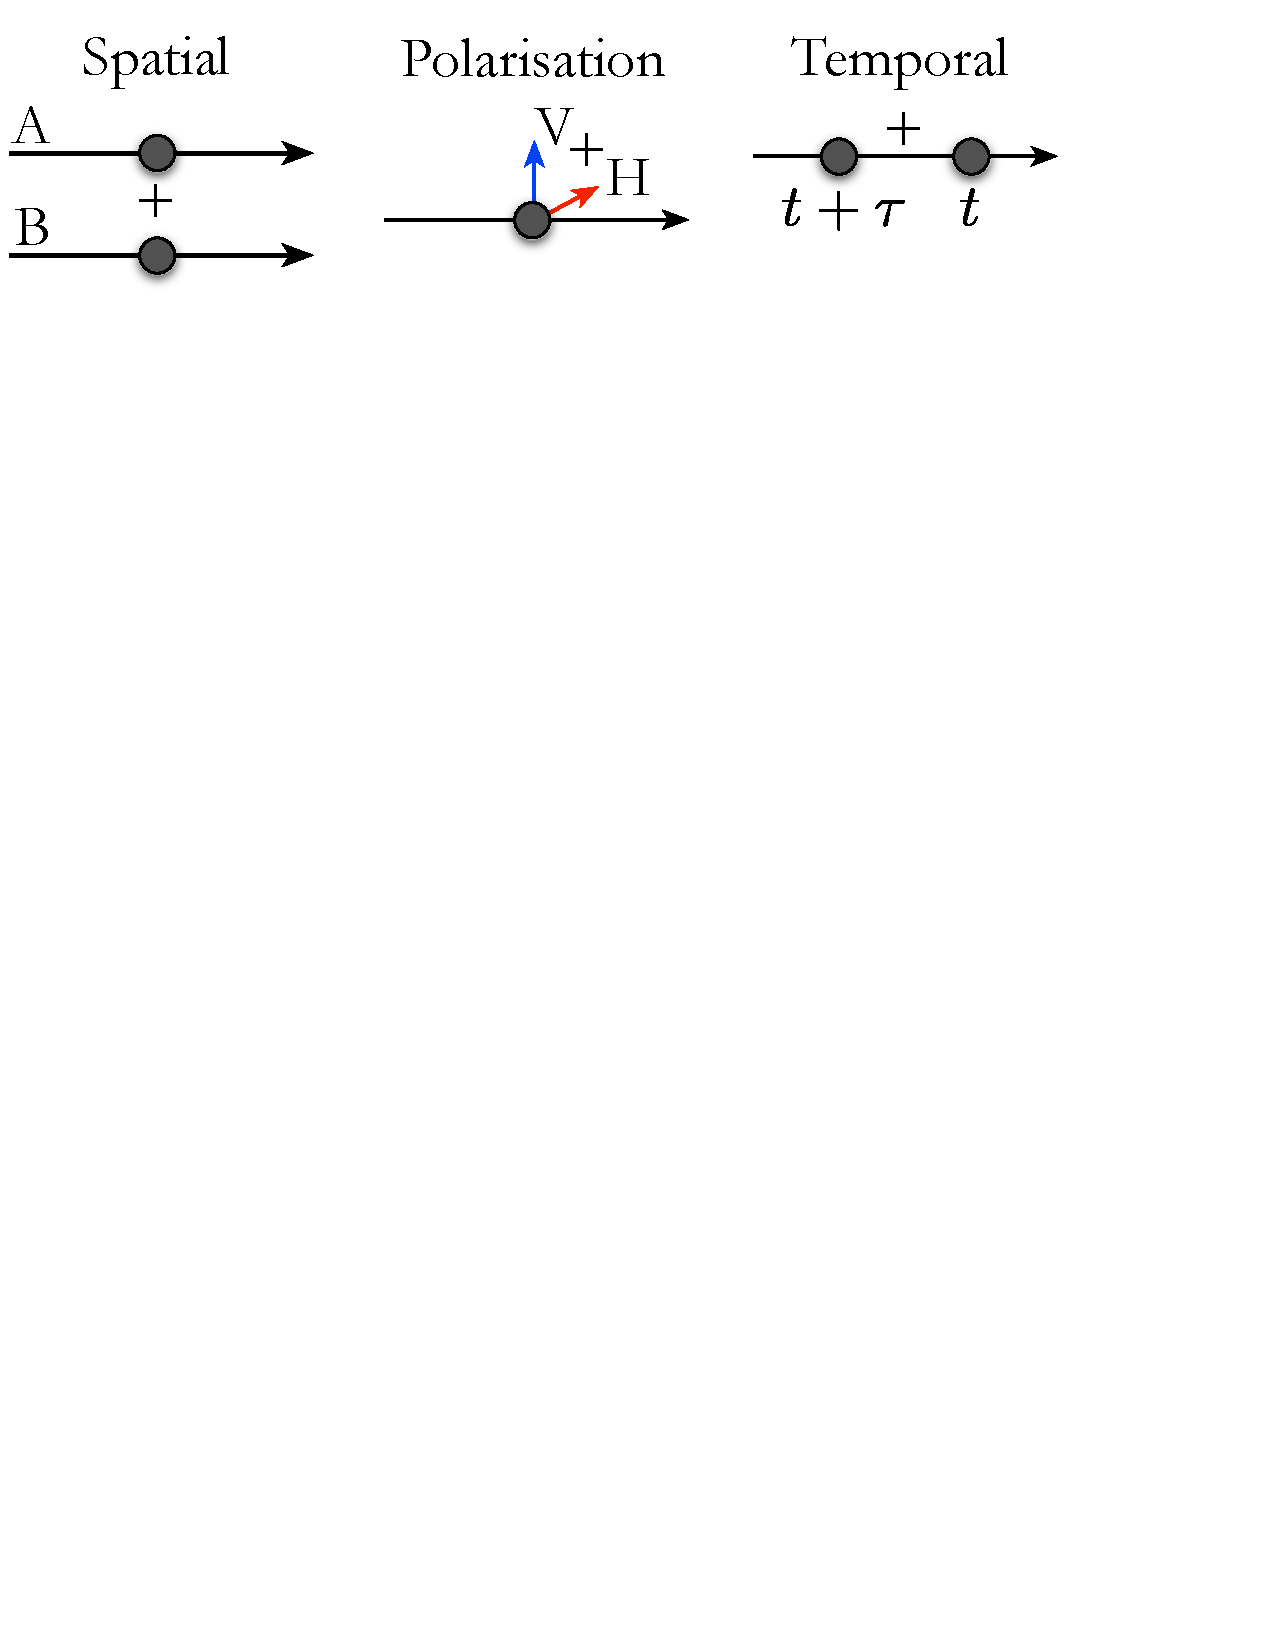
\includegraphics[width=0.15\textwidth]{photonic_qubit_encodings}
\caption{Three approaches to encoding a single qubit using a single photon, via a superposition across two spatial ($A$ and $B$), polarisation ($V$ and $H$) or temporal ($t$ and \mbox{$t+\tau$}) modes.} \label{fig:photonic_qubit_encodings}
\end{figure}

Conversion between polarisation and dual-rail encoding is straightforward and deterministic using standard optical components, as described in Fig.~\ref{fig:pol_to_dual_conv}.

\begin{figure}[!htb]
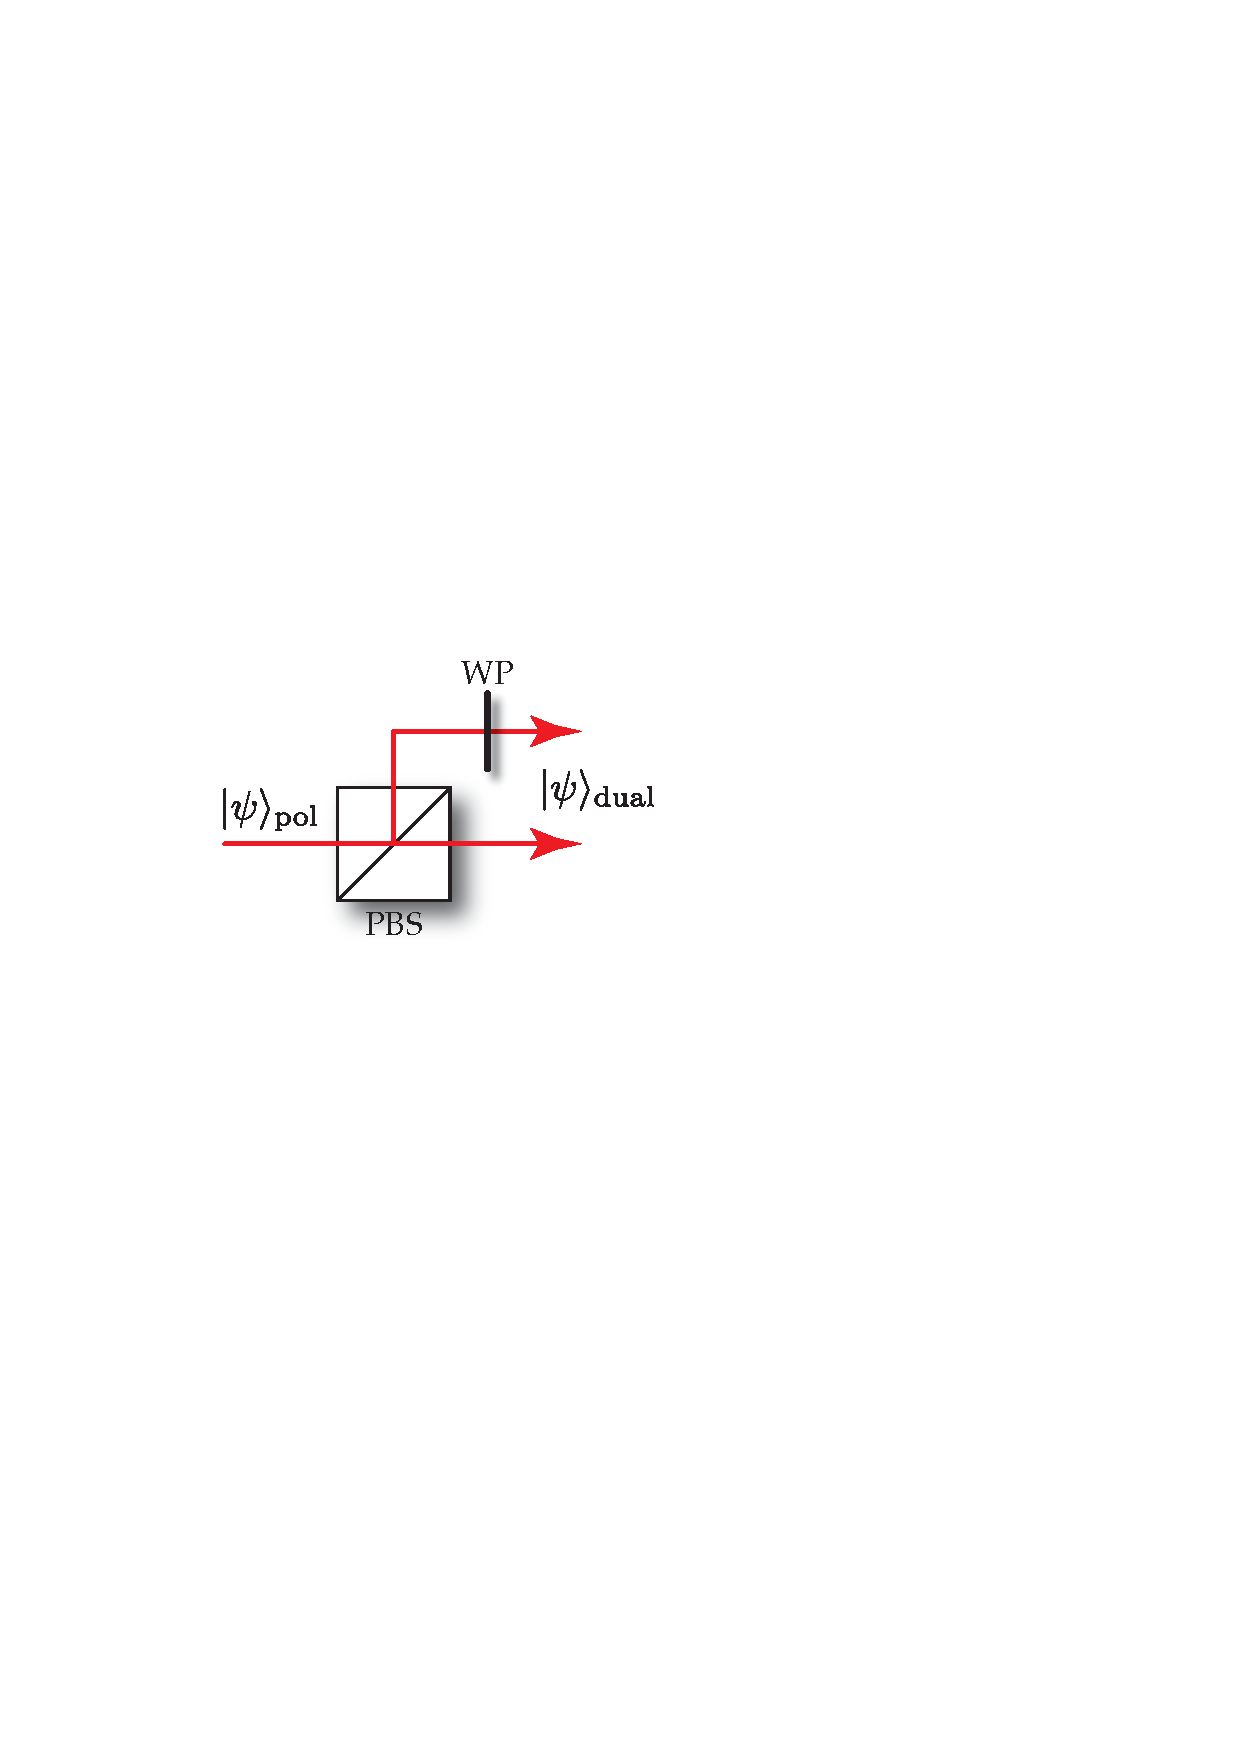
\includegraphics[width=0.3\textwidth]{pol_to_dual_conversion}
\caption{Conversion from single-photon polarisation encoding to dual-rail encoding, using a polarising beamsplitter (PBS) and wave-plate (WP). The PBS separates the polarisation components into two distinct spatial modes. The WP then rotates the polarisation of one of the spatial modes such that it has the same polarisation as the other. Conversion from dual-rail to polarisation encoding is just the reverse of this procedure.} \label{fig:pol_to_dual_conv}\index{Polarising beamsplitters}
\end{figure}

Note that polarisation encoding requires a single spatial mode per qubit, whereas dual-rail encoding requires two. Polarisation encoding brings with it the advantage that arbitrary single-qubit operations may be implemented using wave-plates, which maintain coherence between the basis states extraordinarily well. In dual-rail encoding, on the other hand, single-qubit operations are implemented using beamsplitter operations between the two spatial modes, which must be interferometrically stable, since consecutive single-qubit operations yields Mach-Zehnder (MZ) interference \cite{bib:Zehnder1, bib:Zehnder2}\index{Mach-Zehnder (MZ) interference}, to be discussed in detail in Sec.~\ref{sec:MZ_inter}.

Single-photon encodings are extremely important, as they form the basis for universal linear optics quantum computing (Sec.~\ref{sec:KLM_univ}), \textsc{BosonSampling} (Sec.~\ref{sec:BS}) and quantum walks (Sec.~\ref{sec:QW}). They are also the simplest optical states for representing single qubits.

%
% Photon-number
%

\subsection{Photon-number} \index{Photon-number encoding}

Of course, the photon-number degree of freedom needn't be limited to 0 or 1 photons. By fully exploiting the photon-number degree of freedom, we can encode a qudit\footnote{A $d$-level system, as opposed to a qubit's two levels.}\index{Qudits} of arbitrary dimension into a single optical mode,
\begin{align} \label{eq:number_qudit}
\ket\psi_\mathrm{qudit} \equiv \sum_{n=0}^\infty \alpha_n \ket{n}.
\end{align}
This may give the impression that a single optical mode has infinite information capacity. Needless to say, this sounds too good to be true, and it is. Loss decoheres photon-number-encoded states exponentially with photon-number, since for large photon-number the probability of a number state retaining its photon-number exponentially asymptotes to zero. So although in principle we can encode an $\infty$-level qudit, the moment any non-zero loss is introduced, this exponential dependence destroys the state (Sec.~\ref{sec:eff_err}).

While photon-number encoding can be useful for communications purposes, it is not very practical for quantum information processing tasks, since operations between basis states are not energy preserving, with each basis state having energy \mbox{$E=n\hbar\omega$}, where $\omega$ is frequency, and $\hbar$ is Planck's constant. Thus, qudit operations would need to be active processes.

%
% Spatio-Temporal Qudit Encoding
%

\subsection{Spatio-temporal} \label{sec:spatio_temporal} \index{Spatio-temporal encoding}

Completely independent of the photon-number degree of freedom, are the spatio-temporal degrees of freedom, which encode the spatial, temporal, and spectral/temporal structure of photons. In the temporal domain, for example, we could define the temporal structure of a single photon as,
\begin{align}
\ket\psi_\mathrm{temporal} = \int_{-\infty}^\infty \psi(t) \hat{a}^\dag(t)\,dt\,\ket{0},
\end{align}
where $\hat{a}^\dag(t)$ is the time-specific photonic creation operator, and $\psi(t)$ is the temporal distribution function \cite{bib:RohdeFreqTemp05}.

Alternately, we can define \textit{mode operators} \cite{bib:RohdeMauererSilberhorn07}\index{Mode operators}, which are mathematically equivalent to creation operators, but create photons with a specific temporal envelope,
\begin{align}
\hat{A}^\dag_\psi &= \int_{-\infty}^\infty \psi(t) \hat{a}^\dag(t)\,dt, \nonumber \\
\ket\psi_\mathrm{temporal} &= \hat{A}^\dag_\psi \ket{0}.
\end{align}
Mode operators commute, inheriting this property directly from photonic creation operators,
\begin{align}
\left[\hat{A}^\dag_{\psi_1},\hat{A}^\dag_{\psi_2}\right]=0.
\end{align}

Now by defining an orthonormal basis of temporal distribution functions, $\{\xi_i\}$, such that,
\begin{align} \label{eq:spec_orth_def}
\bra{0} \hat{A}_{\xi_i} \hat{A}^\dag_{\xi_j}\ket{0} = \delta_{i,j},
\end{align}
we can encode a qudit of arbitrary dimension into the spatio-temporal degrees of freedom,
\begin{align}
\ket\psi_\mathrm{qudit} \equiv \sum_{i=0}^\infty \alpha_i \hat{A}^\dag_{\xi_i} \ket{0}.
\end{align}

This encoding allows a qudit of arbitrary dimension to be encoded into a single spatial mode. Again, however, summing to infinity is somewhat fanciful, given any physically realistic spatio-temporal error model, such as an imperfect frequency response in the channel, e.g a bandpass response of an optical fibre or photo-detector.

%
% Time-Bins
%

\subsection{Time-bins} \label{sec:time_bin} \index{Time-bin encoding}

In time-bin encoding we define our basis of modes (whether it be qubits or higher-dimensional qudits\index{Qudits}) as distinct, non-overlapping time-bins, which are localised wave-packets in the temporal degree of freedom, each separated from the next by some fixed interval $\tau$. This can be considered a special case of spatio-temporal encoding\index{Spatio-temporal encoding}, where the basis mode functions satisfy the relation,
\begin{align}
\xi_{j}(t) = \xi_0(t-j\tau),
\end{align}
as well as the usual orthonormality constraints. Here $\tau$ is sufficiently large, and $\xi_i(t)$ sufficiently temporally localised, that the temporal modes are orthogonal as per Eq.~(\ref{eq:spec_orth_def}).

Time-bin encoding arises naturally in architectures where the photon source driving the system is operating at a high repetition rate\index{Repetition rate}, $R$, in which case \mbox{$\tau=1/R$}. Architectures for optical quantum computing have been described \cite{bib:RohdeLoop15, bib:RohdeUnivLoop15}, and experimentally demonstrated \cite{???}, based entirely on time-bin encoding.

These schemes can be very resource efficient, since a single source operating at high repetition rate can replace an entire bank of distinct sources that would ordinarily be required in spatial architectures. Similarly, a single time-resolved detector, with resolution at least $\tau$, can replace a bank of detectors operating in parallel. And only a single spatial mode is required to store an arbitrary number of qubits/qudits, so long as it is long enough to support the entire pulse-train -- at least $2n\tau$ for $n$ qubits.

In the schemes of \cite{bib:RohdeLoop15, bib:RohdeUnivLoop15}, entire optical quantum computing protocols can be efficiently constructed using only a single source, a single detector, two delay-lines, and three dynamically-controlled beamsplitters, irrespective of the size of the computation, an enormous resource saving compared to traditional spatial encodings. Furthermore, in these schemes, there is only a single point of interference, greatly simplifying optical interferometric alignment, which would ordinarily require simultaneously aligning a large number of optical elements, as many as $O(m^2)$ elements for an $m$-mode network \cite{bib:Reck94}.

%
% Thermal State Encoding
%

\subsection{Thermal states} \index{Thermal state encoding}\label{sec:thermal_states}

In some quantum protocols, although the inner workings may be quantum mechanical in nature, the inputs and outputs needn't capture any quantum coherence -- sometimes \textit{classical} information is sufficient for communications. As discussed above, coherent states are the archetypal example of this, and this is in fact the norm in present-day classical fibre-optic communication, where coherent states prepared from laser diodes are employed.

Another, and even simpler option, is thermal states. These are obtained by fully dephasing a coherent state, retaining the amplitudes, while nullifying all the coherence terms,
\begin{align}
\hat\rho_\mathrm{thermal}(\alpha) = e^{-|\alpha|^2} \sum_{n=0}^\infty \frac{|\alpha|^2}{n!}\ket{n}\bra{n}.
\end{align}

Thermal states can encode classical information into their amplitudes, polarisations, or time-bins, as before. The advantage of this type of encoding is that thermal states are trivial to prepare and measure (a normal incandescent lightbulb produces thermal states of light). However, they are purely classical states, do not undergo interference with one another, and are therefore useless for, for example, entangling qubits via which-path erasure, any other type of coherent interferometric process, or for representing quantum information such as qubits.

%
% Phase-Space
%

\subsection{Phase-space} \label{sec:exotic} \index{Phase-space encoding}

When encoding information optically, we needn't restrict ourselves to photon-number states. We also have a lot of flexibility to encode information in phase-space using continuous-variable (CV) states, where phase and amplitude relations encode quantum information \cite{bib:CahillGlauber69}.

In phase-space, the most common representations of optical states are in terms of quasi-probability functions\index{Quasi-probability functions}\footnote{The term `quasi-probablity' arises because in some regimes (for example, strictly non-negative $P$-functions), the function has a true probabilistic interpretation. However this interpretation breaks down for any negativity in the $P(\alpha)$, since negative probabilities have no meaningful classical interpretation.}:
\begin{itemize}\index{$P$-function}\index{$Q$-function}\index{Wigner function}
\item $P$-function: represents a state as a quasi-mixture of coherent states. When the $P$-function is strictly non-negative, it can be interpreted as a perfect classical mixture of coherent states. However, with any negativity this classical interpretation breaks down, hence `quasi'-probability. In general, the $P$-function representation for a state is not unique.
\begin{align}
\hat\rho = \int\!\!\!\int P(\alpha) \ket{\alpha}\bra{\alpha} d^2\alpha.
\end{align}
\item $Q$-function: represents a state in terms of its overlap with the complete set of all coherent states, which form an over-complete basis.
\begin{align}
Q(\alpha) = \frac{1}{\pi} \bra{\alpha}\hat\rho\ket{\alpha}.
\end{align}
\item Wigner function: also has a quasi-probability interpretation, and negativity is qualitatively associated with `quantumness'. The Wigner function of a state is unique, and isomorphic to the density operator, making it perhaps the most useful phase-space representation for quantum states of light.
\begin{align}
W(x,p) = \int e^{ips/\hbar} \left\langle{x-\frac{s}{2}}\right| \hat\rho \left|{x+\frac{s}{2}}\right\rangle ds.
\end{align}
\end{itemize}
These representations, whilst entirely equivalent to a photon-number basis representation, are far easier to work with for many types of states. Most notably, Gaussian states are conveniently represented and manipulated using phase-space representations.

%
% Coherent States
%

\subsubsection{Coherent states} \label{sec:coherent_state_enc} \index{Coherent state encoding}

As the most trivial CV encoding of quantum information, consider coherent states. These are particularly useful since they are pure states, with well defined coherence relationships, and are closely approximated by laser sources, and therefore readily available in the lab.

A coherent state, $\ket\alpha$, is parameterised by a single complex parameter, $\alpha$, given by a phase and amplitude,
\begin{align}\index{Coherent states}
\ket{\alpha} = e^{-\frac{|\alpha|^2}{2}} \sum_{n=0}^\infty \frac{\alpha^n}{\sqrt{n!}} \ket{n}.
\end{align}
Fig.~\ref{fig:coherent_state_encoding} illustrates the phase-space representation for two approximately orthogonal coherent state basis states.

\begin{figure}[!htb]
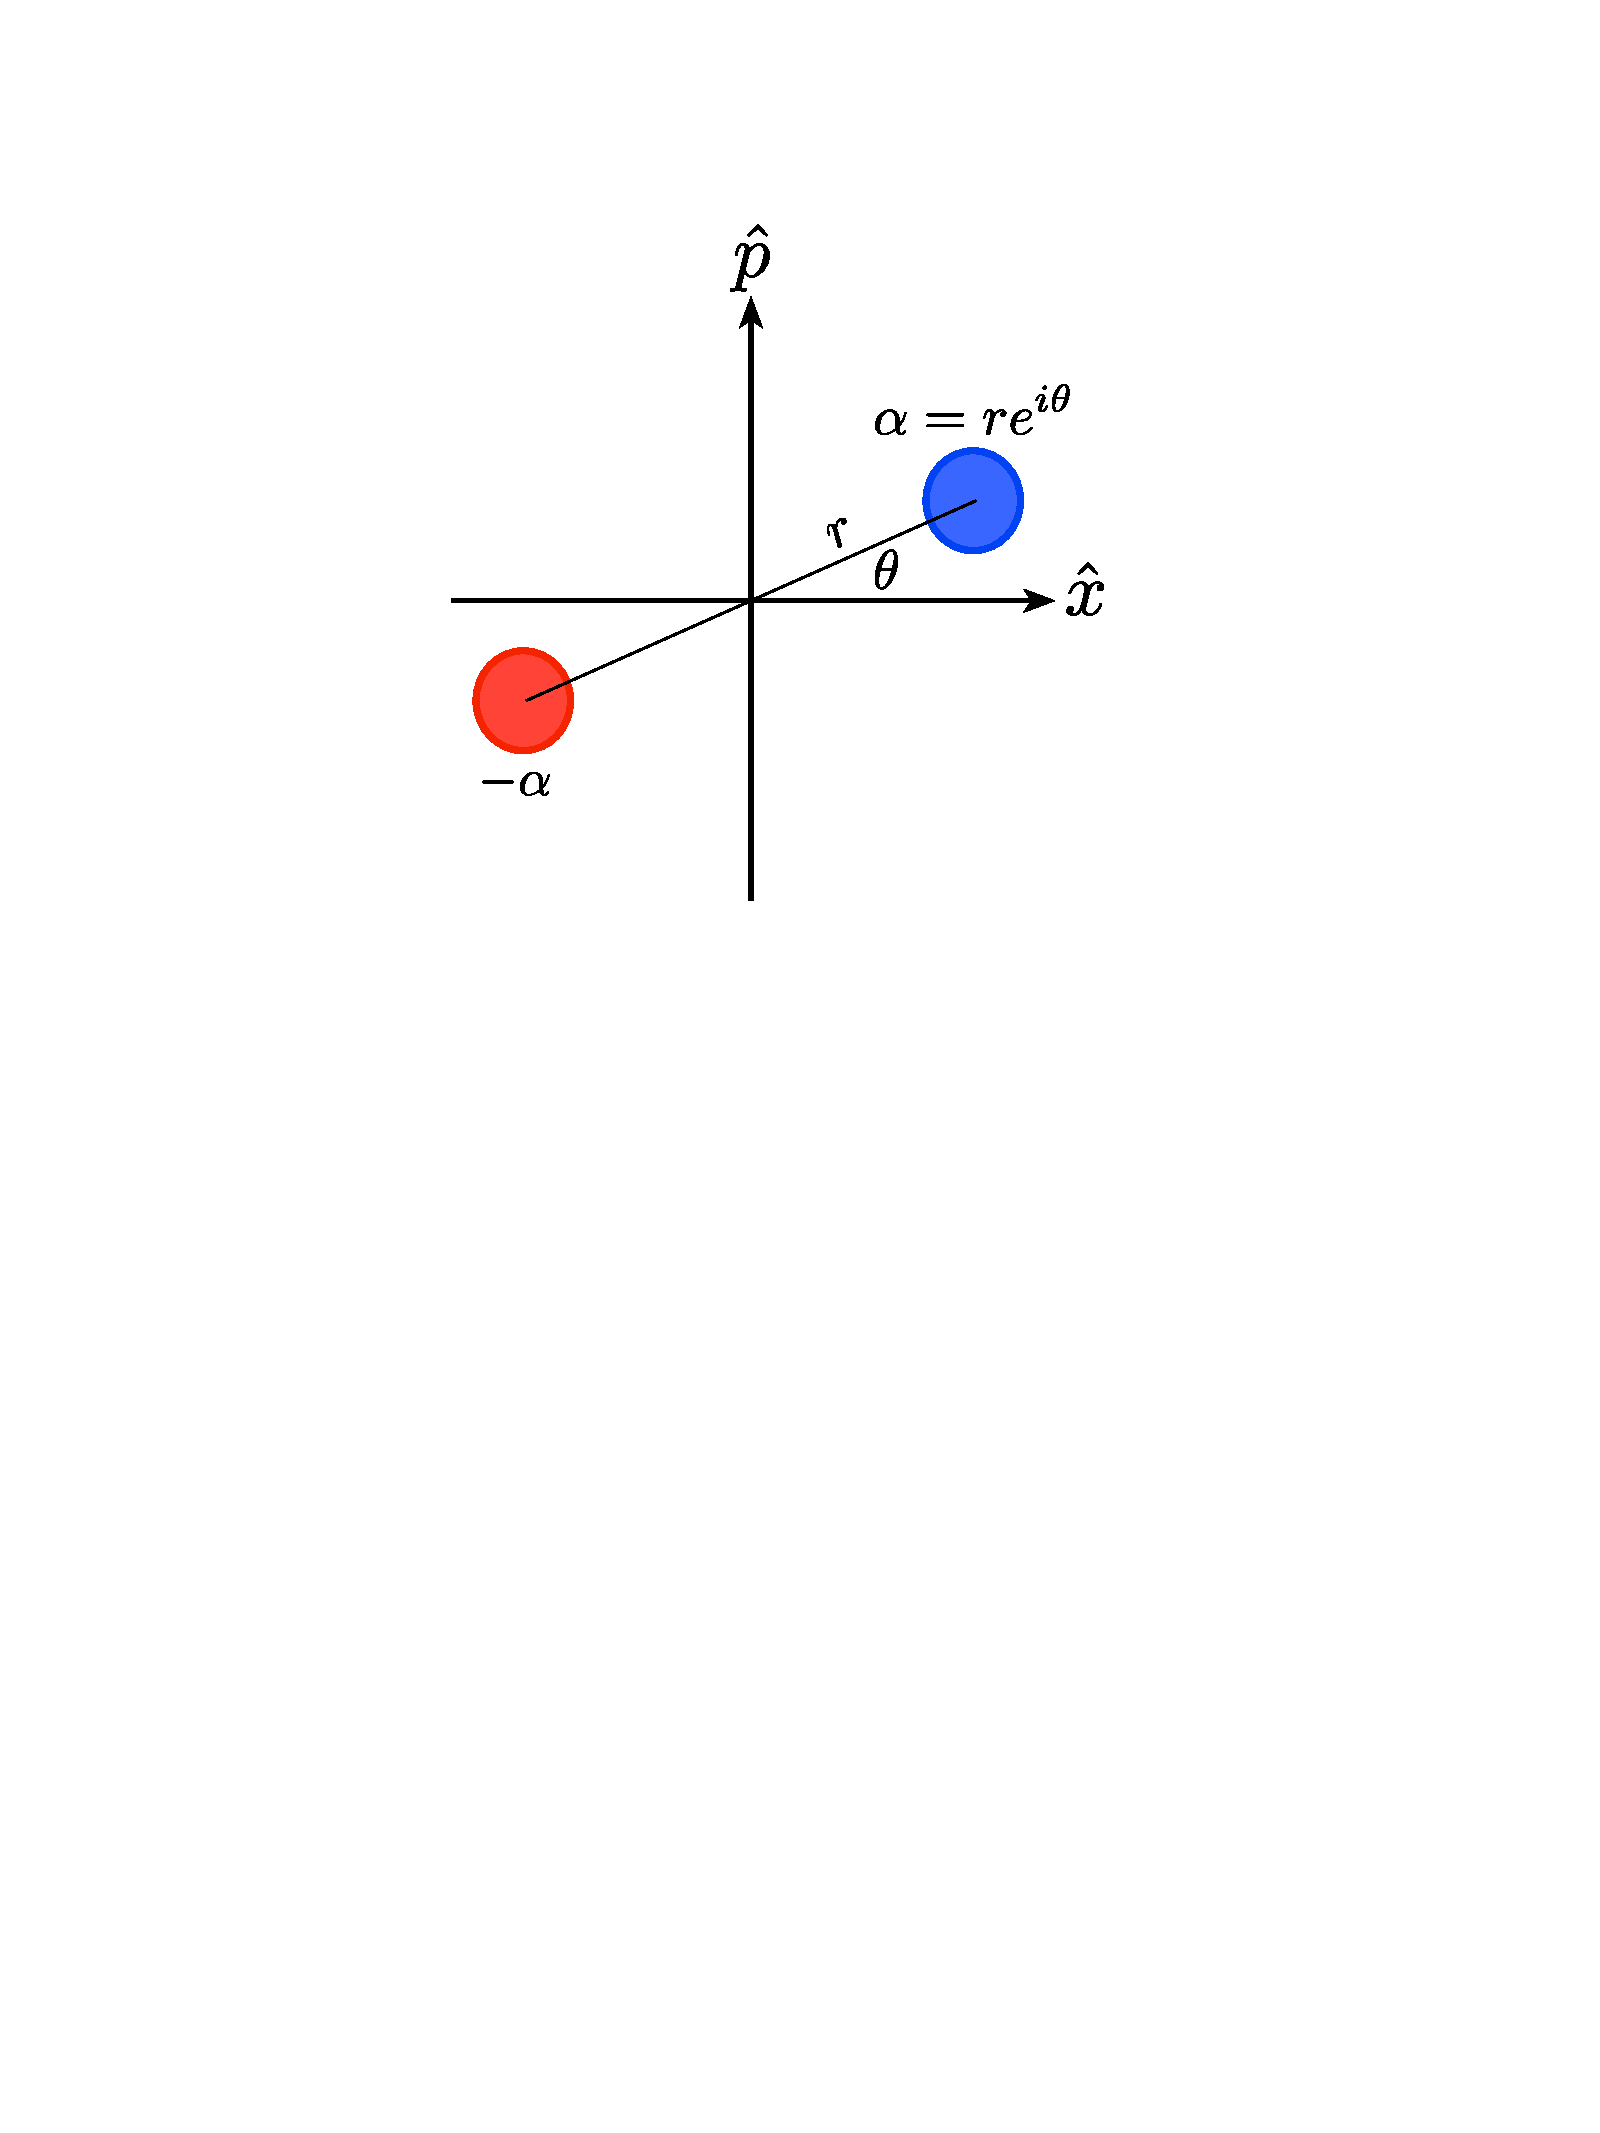
\includegraphics[width=0.4\textwidth]{coherent_state_encoding}
\caption{Phase-space representation of a coherent state with complex amplitudes $\pm\alpha$. For sufficiently large amplitude one can approximate orthogonality, enabling a qubit encoding.} \label{fig:coherent_state_encoding}	
\end{figure}

By manipulating these parameters, information can be encoded into coherent states. We could, for example, define two coherent states of opposite phase to represent qubit basis states,
\begin{align}
\ket{0} &\equiv \ket{\alpha}, \nonumber \\
\ket{1} &\equiv \ket{-\alpha}.
\end{align}
Note, however, that this representation for qubits is only approximate, since the two basis states are not perfectly orthogonal,
\begin{align}
\langle -\alpha|\alpha \rangle = e^{-2|\alpha|^2},
\end{align}
which is non-zero for any finite $\alpha$, whereas for ideal qubits we require \mbox{$\langle 0|1\rangle = 0$}. However, for large $\alpha$, $\ket{\pm\alpha}$ closely approximate orthogonality.

This representation for qubits using coherent states is easily generalised to qudits by considering coherent states orbiting the origin of phase-space at equal angular intervals of \mbox{$2\pi/d$}, for a $d$-level qudit. The $k$th qudit basis state is then,
\begin{align}
\ket{k}_d = \ket{e^{ik/d}\alpha},
\end{align}
for \mbox{$k=0,\dots,d-1$}, where again the basis states are non-orthogonal, but closely approximate orthogonality for large $\alpha$.

Note that despite being pure states, with well-defined coherence, coherent states are considered classical, as they are unable to encode quantum information. That is, the coherence relationships cannot be exploited for the encoding of qubits or qudits.

Coherent states are useful in that they are easy to prepare using modern lasers, including laser diodes, and by turning up the amplitude can be transmitted over long distances, with loss not affecting quantum coherence, only the amplitude (Sec.~\ref{sec:eff_err}).

%
% Cat States
%

\subsubsection{Cat states} \label{sec:cat_enc} \index{Cat state encoding}\index{Cat states}

Another type of CV state, which can in fact encode quantum information, is superpositions of coherent states (colloquially known as `cat' states), with the encoding \cite{???},
\begin{align}
\ket{0} &\equiv \frac{1}{\sqrt{2(1+e^{-2|\alpha|^2})}} (\ket{\alpha}+\ket{-\alpha}) \nonumber \\
&= \ket{\mathrm{cat}_+(\alpha)},\nonumber \\
\ket{1} &\equiv \frac{1}{\sqrt{2(1-e^{-2|\alpha|^2})}}(\ket{\alpha}-\ket{-\alpha}) \nonumber \\
&= \ket{\mathrm{cat}_-(\alpha)}.
\end{align}
These two basis states contain strictly even or odd photon-number terms respectively (i.e they have well-defined parity), implying that, unlike coherent states, they are always orthogonal, regardless of amplitude,
\begin{align}
\langle\mathrm{cat}_+(\alpha)|\mathrm{cat}_-(\alpha)\rangle = 0 \,\,\forall\,\alpha,
\end{align}
making them directly appropriate for qubit encoding, even for weak coherent amplitudes.

Unfortunately, cat states are notoriously difficult to prepare, and extremely sensitive to loss (Sec.~\ref{sec:single_phot_enc}) and dephasing (Sec.~\ref{sec:dephasing_error}). This arises because loss of a single photon flips the parity of the state to an orthogonal one, meaning that as $\alpha$ increases, the state is exponentially more susceptible to decohering into a mixture of the logical basis states.

However, modulo these difficulties, with a resource of cat states at one's disposal, universal quantum computation may be realised using post-selected linear optics \cite{bib:JeongRalph05, bib:Gilchrist04}.

%
% Squeezed States
%

\subsubsection{Squeezed states}\index{Squeezed states}

Coherent state encoding can be regarded as encoding via the displacement operator, Eq.~(\ref{eq:disp_op}), which implements translations in phase-space. Alternately, we can encode via the squeezing operator, Eq.~(\ref{eq:sq_op}), which implements dilations about an axis in phase-space. Squeezing the vacuum state along the $\hat{x}$ or $\hat{p}$ directions yields two states that are approximately orthogonal for large squeezing amplitudes, as shown in Fig.~\ref{fig:squeezed_state_encoding}. Thus, with sufficient squeezing they can be used as a basis for approximately encoding a qubit. This encoding can be exploited for full universal quantum computing, as was introduced in Sec.~\ref{sec:CV_QC}.

%
% Non-Optical Encoding
%

\subsection{Non-optical encoding}\index{Non-optical encodings}

In a non-optical context, the elementary unit of quantum information -- the qubit -- can be naturally encoded into any system with a natural or engineered two-level structure. This actually encompasses a broad range of possibilities, including, amongst many others:
\begin{itemize}
\item \index{2-level systems}Two-level atoms: let two distinct electron energy levels, with long lifetimes, represent the two logical basis states.
\item \index{$\lambda$-configuration systems}$\lambda$-configuration atoms: atoms with two degenerate ground states, which encode the logical qubit, and an additional excited state, which may be transitioned to upon excitation from only one of the ground states. Relaxation from the excited state enables optical coupling via the emitted photon.
\item \index{Quantum dots}Quantum dots: are essentially artificial atoms, which can be engineered with custom band-structures, allowing two- or higher-level qudits to be easily fabricated.
\item \index{Nitrogen-vacancy (NV) centres}Nitrogen-vacancy (NV) centres: are a type of point defect in diamond, which has a very well defined energy level structure that may be utilised to represent qubits.
\item \index{Atomic ensembles}Atomic ensembles: encode quantum information similarly to a single atom, except that the excitation is a \textit{collective} one, in superposition across all the atoms in the ensemble.
\item \index{Superconducting rings}Superconducting rings: a superposition of current flow direction in a superconducting ring represents the two logical basis states.
\item \index{Trapped ions}Trapped ions: qubits are encoded into stable electronic states of electromagnetically trapped ions.
\end{itemize}

Clearly the non-optical elements in a quantum network must somehow interface with optical states, such that communication is facilitated. This is discussed later in Sec.~\ref{sec:opt_inter}.